\chapter{Marco Teórico}
\label{marcoteorico}

%Aquí va una lista:
%\begin{itemize}
    %\item Ingeniería Informática.
    %\item Ingeniería Sonido e Imagen en Telecomunicación.
    %\item Ingeniería Multimedia.
    %\begin{itemize}
         %\item Mención: Creación y ocio digital.
         %\item Mención: Gestión de Contenidos.
    %\end{itemize}
%\end{itemize}




\begin{figure}
\begin{center}
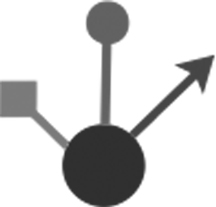
\includegraphics[scale=0.25]{imagenes/logoim.jpg}
\caption{Logo de Ingeniería  Multimedia.}
\label{logo_im}
\end{center}
\end{figure}

\begin{figure}
\begin{center}

\includegraphics[scale=0.25]{imagenes/logoeps.jpg}
\caption{Logo de la EPS.}
\label{logo_eps}
\end{center}
\end{figure}

\section{El marketing digital en la web}

 \cite{listing_packagge} y en \cite{heinz1listings}.

Otro ejemplo, ahora para mostrar código PHP, sería escribir en tu fichero \LaTeX lo siguiente:
\begin{verbatim}
 \begin{lstlisting}[style=PHP, caption={ejemplo código PHP},label=PHP_code]
 /* 
Ejemplo de código en PHP para escribir tu primer programa en este lenguaje
Copia este código en tu ordenador y ejecútalo
*/
<html>
  <head>
    <title>Prueba de PHP</title>
  </head>
  <body>
    <?php echo '<p>Hola Mundo</p>'; ?> //esto lo escribe TODO el mundo
  </body>
</html>
 \end{lstlisting}
\end{verbatim}
 
 y el resultado es: (ver listado \ref{PHP_code})
 